\chapter{Diagrama de Gantt}

El diagrama de Gantt es una herramienta que utilizan los equipos para ver de forma visual las tareas que hay que realizar, con el tiempo estimado para cada una.\\

En nuestro caso, hemos divido el diagrama por semanas a lo largo de los meses de octubre, noviembre y diciembre. Cada tarea es una user storie que deberá estar implementada en el tiempo indicado.

\begin{figure}[h]
    \centering
    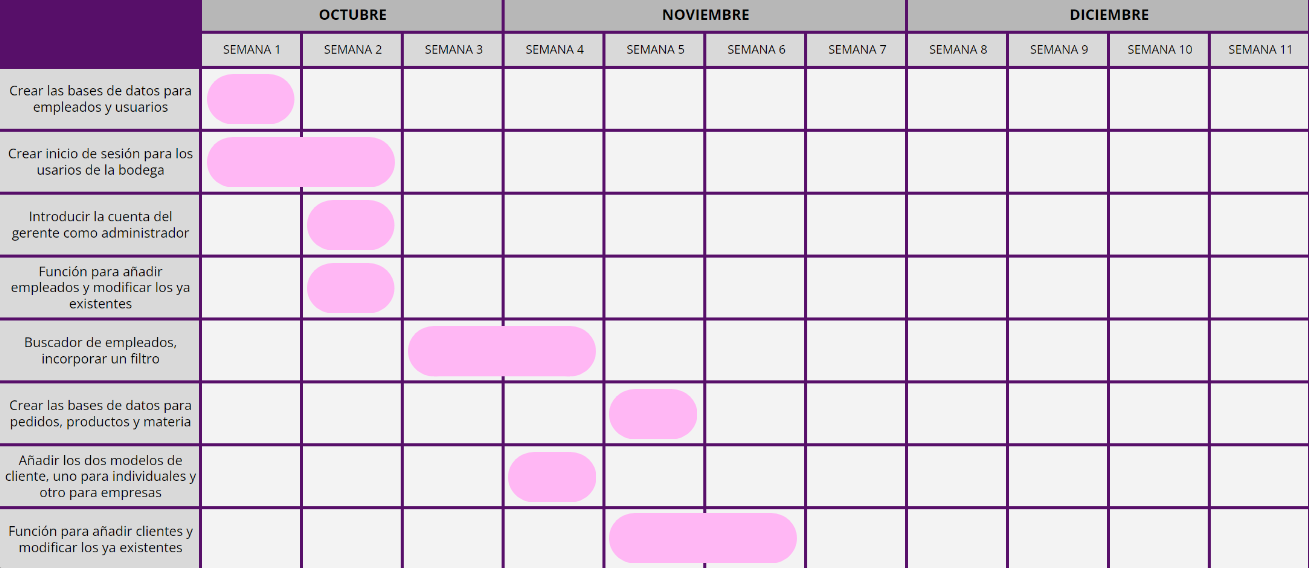
\includegraphics[width=1\textwidth]{figures/gantt-1.png}
    \caption{Primera parte del diagrama de Gantt}
    \label{fig:gantt1}
\end{figure}

\begin{figure}[h]
    \centering
    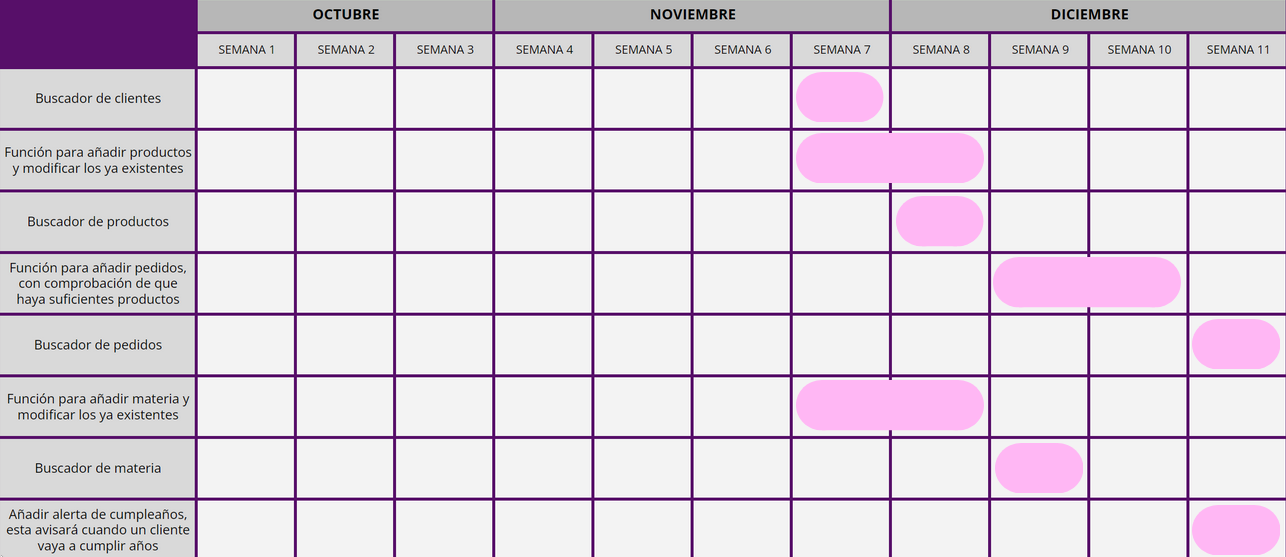
\includegraphics[width=1\textwidth]{figures/gantt-2.png}
    \caption{Segunda parte del diagrama de Gantt}
    \label{fig:gantt2}
\end{figure}
